\documentclass{article}

% if you need to pass options to natbib, use, e.g.:
%     \PassOptionsToPackage{numbers, compress}{natbib}
% before loading neurips_2018

% ready for submission
% \usepackage{neurips_2018}

% to compile a preprint version, e.g., for submission to arXiv, add add the
% [preprint] option:
%     \usepackage[preprint]{neurips_2018}

% to compile a camera-ready version, add the [final] option, e.g.:
     \usepackage[final]{neurips_2018}

% to avoid loading the natbib package, add option nonatbib:
%     \usepackage[nonatbib]{neurips_2018}

\usepackage[utf8]{inputenc} % allow utf-8 input
\usepackage[T1]{fontenc}    % use 8-bit T1 fonts
\usepackage{hyperref}       % hyperlinks
\usepackage{url}            % simple URL typesetting
\usepackage{booktabs}       % professional-quality tables
\usepackage{amsfonts}       % blackboard math symbols
\usepackage{nicefrac}       % compact symbols for 1/2, etc.
\usepackage{microtype}      % microtypography

\usepackage{geometry, amsmath, amsthm, latexsym, amssymb, graphicx, caption, float, graphbox, fontawesome}

\newcommand{\cited}[1]{\textsuperscript{\ref{itm:#1}}}

\title{Identifying Transcription Unit Structure from Rend Sequencing Data}

\author{
  Travis Horst \\
  thorst@stanford.edu
}

\begin{document}
% \nipsfinalcopy is no longer used

\maketitle

\begin{abstract}
The goal of this project is to use sequencing data to identify transcription unit initiation and termination sites within a genome to determine which genes are expressed together. Although partially known, identifying all transcription units in an organism can help create more accurate models of biologic behavior by better capturing interactions between coexpressed genes leading to higher predictive capacity. Unsupervised and supervised methods were used to identify structure from transcript sequencing data. Supervised learning methods performed better at identifying transcription start and stop sites and avoiding false predictions; however, they did not generalize well to the test set.
\end{abstract}

\section{Introduction}
In bacteria, many genes are expressed together on the same RNA transcript called a transcription unit (TU). Identifying all possible TUs can play a role in better understanding biology as related genes are typically expressed together.  Ultimately, these transcripts are translated to proteins which carry out much of the functionality in cells so coexpression can have important physiological implications as these proteins interact with each other.  Although many TUs (>3500 for \textit{E. coli}) have been identified and compiled in databases,\cited{ecocyc} there is not an efficient way to determine all of the TUs in an organism.  Sequencing techniques can provide high throughput data of the transcripts in populations of bacteria and recent work (Figure \ref{fig:reads})\cited{lalanne} has shown promise in identifying TUs, claiming the method was able to identify more than 500 5' ends and more than 1000 3' ends (neither precision nor sensitivity were presented because this could include novel sites that were not previously annotated).  The code made available by the group to perform analysis (using peak z-score) was not generally applicable to entire the genome and requires some manual intervention.  Automated analysis of this data across the entire genome would allow progress to be made in improving the predictive capacity of models, such as models for whole cells,\cited{karr} which has far reaching impacts in industry and medicine. Rend sequencing data, as provided in the work by Lalanne \textit{et al.},\cited{lalanne} can provide benefits over other sequencing data as it does not suffer from 3' end bias and shows enrichment at the start and end of TUs as seen by spikes in the read count plots.  With this in mind, the goal of this project is to find a machine learning algorithm that can take the read counts at each position in the genome and predict the locations in the genome where initiation and termination of transcripts occurs.  Unsupervised (DBSCAN and hidden Markov models) and supervised (logistic regression and neural networks) methods were explored.

\section{Dataset and Features}
The dataset comes from Rend sequencing data in \textit{E. coli} from Lalanne \textit{et al}.\cited{lalanne} The raw data input is $X\in \mathbb{R}^{9,279,350\text{x}2}$. The length of the genome is 4,639,675 base pairs with transcripts mapped to each genome location in both the forward and reverse direction for a total of 9,279,350 locations.  For each genome location, there are two values for reads, one for the counts that occur at the 5' end of a transcript and one for counts at the 3' end. 152 locations in the genome were annotated by hand as containing an initiation or termination site.  This was divided into 74 positions for training, 40 positions for validation and 38 positions for testing.  For unsupervised methods, training and validation were grouped together while holding out the same test set.

Some processing of the data is required to better fit assumptions for the algorithms.  For unsupervised learning, the first thing that must be done is to segment the reads into regions that contain multiple genes that are separated by other regions by areas of no reads.  The algorithms used will handle small regions of genes better than the entire genome at once.  An example of this segmentation is shown below in the bottom of Figure \ref{fig:reads}.

\begin{figure}[H]
    \centering
    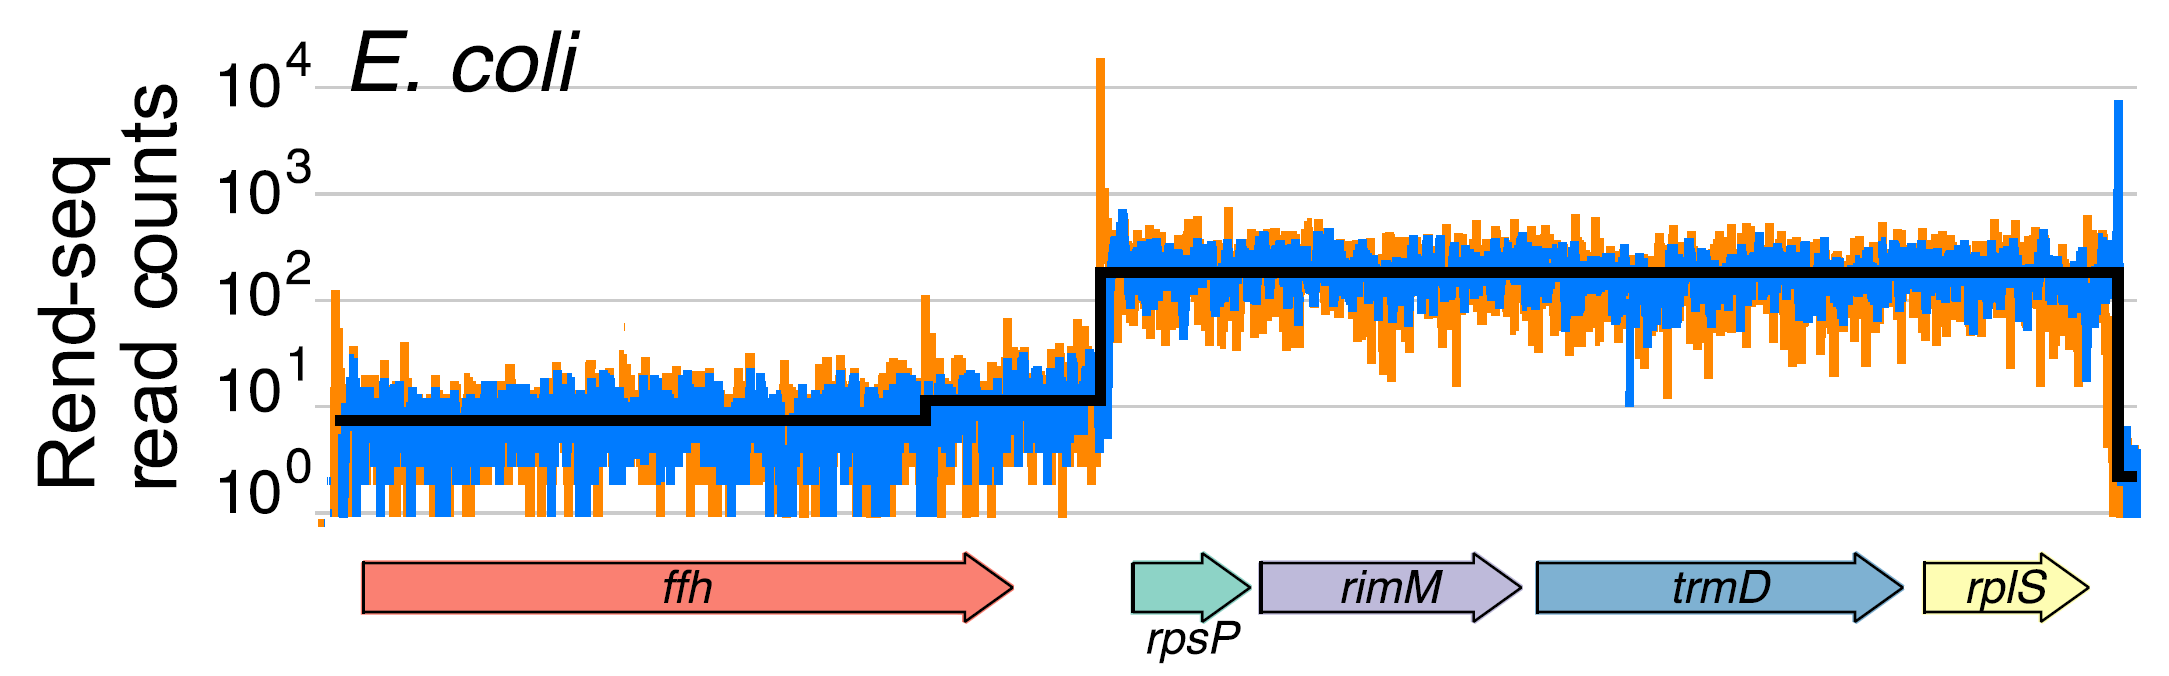
\includegraphics[width=0.6\textwidth]{lalanne_reads.png} \\
    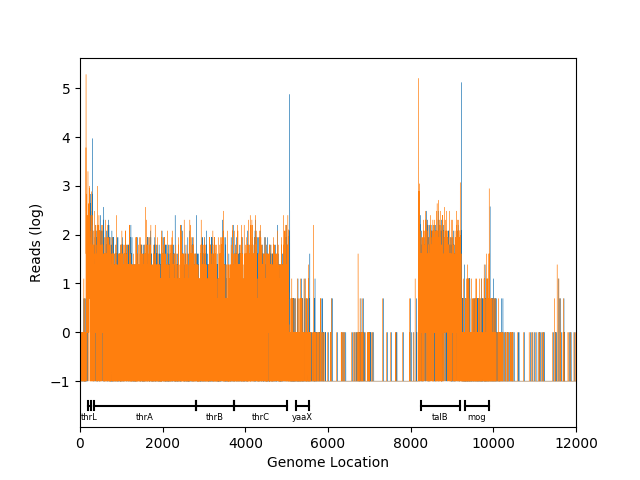
\includegraphics[align=c, width=0.3\textwidth]{both.png} $\boldsymbol{\longrightarrow}$
    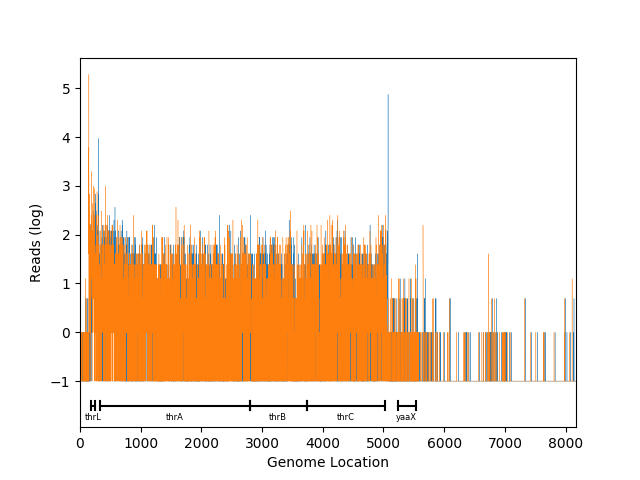
\includegraphics[align=c, width=0.3\textwidth]{0.png} $\boldsymbol{+}$
    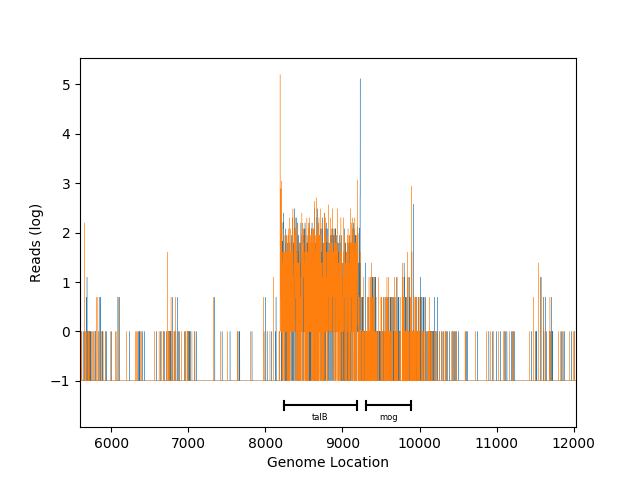
\includegraphics[align=c, width=0.3\textwidth]{1.png}
    \caption{Top: example data with genes. Orange and blue are reads, black indicates TUs.\cited{lalanne}\\ Bottom: example of two read regions before (left of arrow) and after (right of arrow) segmentation.}
    \label{fig:reads}
\end{figure}

The raw data represents counts and follows a Poisson distribution so the data was further processed to transform the distribution to a Gaussian distribution to better fit the assumption made by the hidden Markov model.  Taking a moving average of the reads can transform the data from a Poisson distribution to a Gaussian distribution as illustrated in Figure \ref{fig:distribution}.  This also has the added benefit of encoding additional positional information into each point, which is useful because most neighboring positions will be in the same set of TUs.  Furthermore, a moving average to the left and to the right of a position of interest for each set of reads was taken in some cases to account for the possibility of a shift in expression.

\begin{figure}[H]
    \centering
    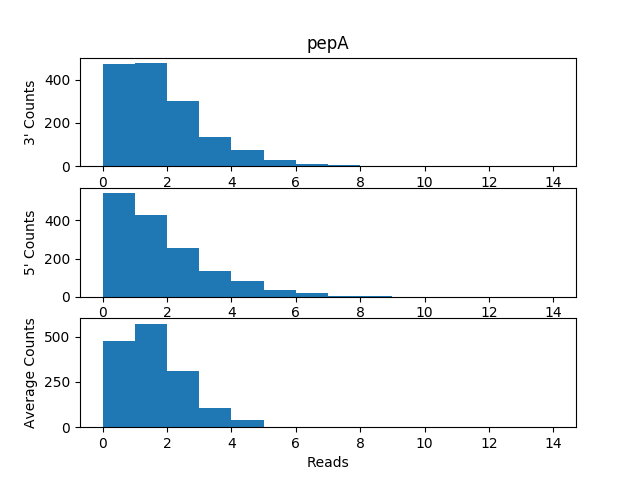
\includegraphics[width=0.35\textwidth]{pepA.png}
    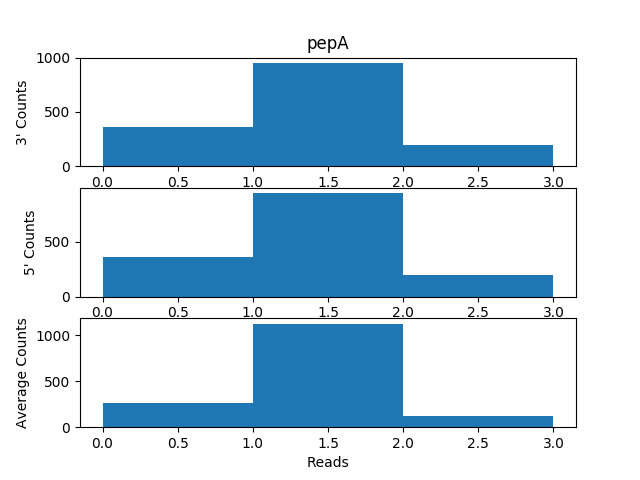
\includegraphics[width=0.35\textwidth]{pepA_ma.png}
    \caption{Transformation of read data for selected gene.  Single location read distribution (Poisson) is shown on the left and the distribution after taking a moving average (Gaussian) is on the right.}
    \label{fig:distribution}
\end{figure}

For the supervised methods, a sliding window along the genome was used to generate samples using reads from consecutive genome positions.  Samples were labeled as an initiation or termination if the window contained one of the annotated locations from above.  A pad value was also specified so that if the peak occurred within the given pad from the edge of the window, the sample was excluded.  This allowed methods to be trained on samples where the peak was only in or near the middle of the window.  Due to class imbalance between normal regions and regions with an initiation or termination, the SMOTE technique\cited{smote} from imblearn\cited{imblearn} was used to oversample the minority classes in some cases.

\section{Methods}

\subsection{Unsupervised Learning}
The first models tried were unsupervised learning methods.  Although some transcription units are already known and well studied, using unsupervised methods could reduce the bias of introducing prior knowledge that might be incorrect or fail to capture unstudied transcription units.

\subsection*{DBSCAN}
The first method implemented was density-based spatial clustering of applications with noise (DBSCAN) clustering.  This method was implemented with the scikit-learn package\cited{sklearn} and calculates the distance between each sample to form clusters of samples that are within a given distance ($\epsilon$) of each other.  Samples that fall in clusters that contain fewer than a specified miniumum number of points are labeled as outliers.  In this case, spikes in read counts are outliers from the rest of the read data and signify the start or end of TUs.

\subsection*{Hidden Markov Model}
This method was selected to provide insight into latent states of the system and implemented with the hmmlearn package.\cited{hmmlearn}  In this case, each TU can be represented by the hidden states with the read counts being the signal that is emitted.  This algorithm allows incorporation of domain knowledge about the system.  Since it is known that the start or end of a TU will correlate with a spike in the read counts on the 3' or 5' end, the transition probabilities can be set up to capture this.  Specifically, there should be two hidden states for each TU, one short one for the transition (spike) and one long one for the length of the TU with transitions only able to progress from one TU to the next.  This means the transition probability matrix, $T$, will be built as shown in Figure \ref{fig:tmat}, where $p_{gene}$ is the probability of seeing a gene (low) and $p_{transition}$ is the probability of leaving a transition (high).
\begin{figure}[H]
    \centering
    \[T = \begin{bmatrix}
    1-p_{gene} & p_{gene} & 0 & 0 & \dots & 0 \\
    0 & 1-p_{transition} & p_{transition} & 0 & \dots & 0 \\
    0 & 0 & 1-p_{gene} & p_{gene} & \dots & 0 \\
    && \vdots \\
    0 & 0 & 0 & 0 & \dots & 1
    \end{bmatrix}\]
    \caption{Transition matrix for hidden Markov model.}
    \label{fig:tmat}
\end{figure}

\subsection{Supervised Learning}
After the poor performance of the unsupervised methods, supervised approaches appeared to be better suited to the problem at hand.  Both methods attempt to classify into three classes - normal, initiation, and termination.  Initiation and termination classes contain an annotated peak in the read data window.

\subsection*{Logistic Regression}
Starting with a simple implementation, a multinomial logistic regression algorithm was implemented from scikit-learn.\cited{sklearn}  With this being a multiclass problem, the multinomial loss was used.  The method will give a probability of a sample, $i$, belonging to a class, $c$, according to Equation \ref{eq:logreg} where $\theta_k$ are parameters learned for each class.  Parameters are learned through gradient ascent with the training data.
\begin{equation}
    \label{eq:logreg}
    p(y^{(i)} = c) = \frac{\exp(\theta_c^\top x^{(i)})}{\sum\limits_{k=1}^3 \exp(\theta_k^\top x^{(i)})}
\end{equation}

\subsection*{Neural Network}
Attempting to improve on logistic regression performance, a fully connected neural network was implemented using Keras\cited{keras} with a TensorFlow\cited{tf} backend.  A sigmoid activation function was used for all of the hidden nodes with a softmax function for the 3 output nodes, which correspond to normal, initiation and termination classes. Various network architectures were explored with between two and four hidden layers containing 5-30 nodes.  With each hidden node, weights and biases are learned through backpropagation with training data.  For each layer, the weight matrix is multiplied by the inputs which then get added to the bias terms. The result is then passed to the activation function to add nonlinearity and the result is passed to the next layer of the network.  The models were trained for 3 epochs as the training accuracy was sometimes low with fewer epochs although validation accuracy over multiple epochs was never checked.

\section{Results}
With this dataset, there is a large class imbalance between the number of normal cases and the number of initiation or termination locations.  Because of this, accuracy is not as useful of a metric and the models should balance a tradeoff between recall and precision where initiation and termination classes are grouped as positive results.  Optimal parameters were selected based on the highest F\textsubscript{1} score across parameters tested.  Equation \ref{eq:f1} shows how F\textsubscript{1} relates recall and precision.  Performance for each method with these selected parameters is summarized in Table \ref{results} with example output for unsupervised methods shown in Figure \ref{fig:unsup} and supervised methods shown in Figure \ref{fig:sup}.

\begin{equation}
    \label{eq:f1}
    F_1 = 2\frac{recall \cdot precision}{recall + precision}
\end{equation}

For DBSCAN, the parameters for the model, $\epsilon$ and $min\_points$, were varied and model performance was assessed with the validation dataset.  The optimal parameters were $\epsilon = 2$ and $min\_points=15$.  As shown in Figure \ref{fig:unsup}, this can identify some peaks in the input data but also gives a large number of false positives.  The same parameters were assessed on the entire set of data even though certain regions in the genome performed better with one set of parameters than another.  This could be due to the range of read counts or the number of genes in a region so some additional processing of the data to normalize the input could improve performance.

For HMM, the data processing approaches were varied to find the best input. This included varying the moving average window and including total counts instead of separate 5' and 3' counts.  The optimal value was surprising a moving average window of 1, which results in a Poisson distribution instead of Gaussian, with separate counts input.  For this model, there were not as many transitions as expected so exploring different transition probabilities might result in better performance.

\begin{figure}[H]
    \centering
    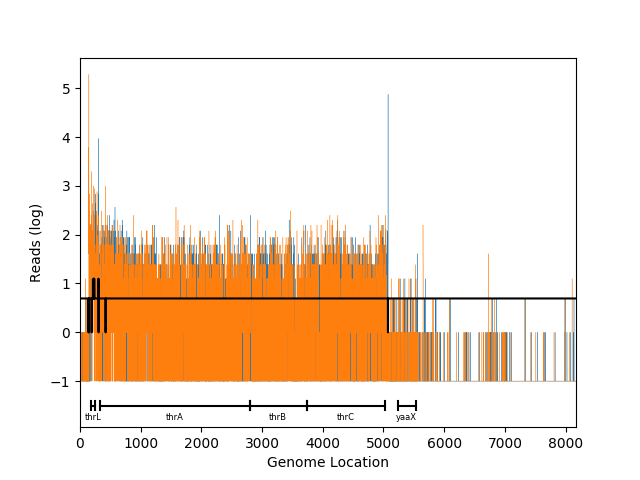
\includegraphics[width=0.4\textwidth]{0_dbscan.png}
    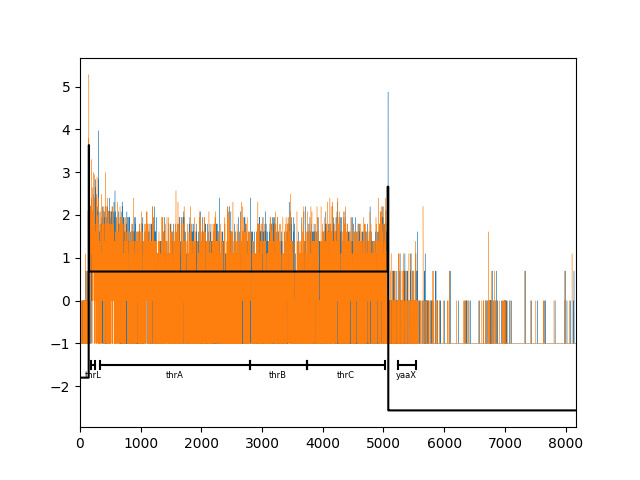
\includegraphics[width=0.4\textwidth]{0_hmm.png}
    \caption{Example output from unsupervised models shown in black with read data in blue and orange.  DBSCAN is on the left and values of 0 indicate outliers, which are positive results.  HMM is on the right and the black trace shows the mean of the hidden state at each position.}
    \label{fig:unsup}
\end{figure}

For logistic regression, several parameters related to data processing were varied.  This included oversampling the minority classes with SMOTE, the moving average window for read counts, the size of the window of reads the algorithm was trying to classify and the pad, which controls the location within the window that the peak needs to appear to be labeled a positive class.  The optimal parameters were no oversampling, no moving average, a window size of 7 with a pad of 3 so training data was labeled as initiation or termination only when the peak was directly centered in the window.

\begin{figure}[H]
    \centering
    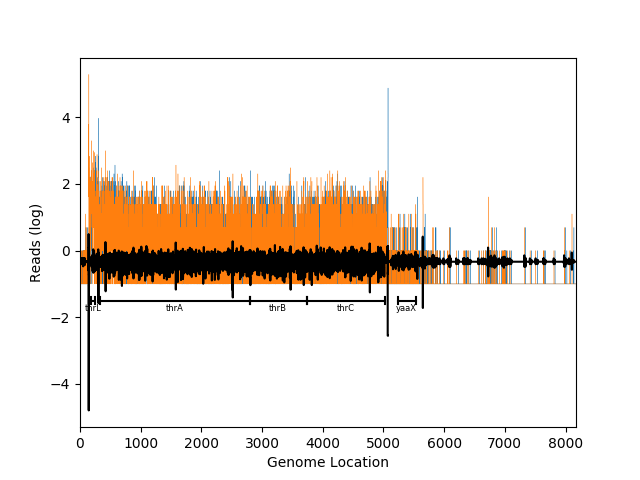
\includegraphics[width=0.4\textwidth]{0_logreg_init.png}
    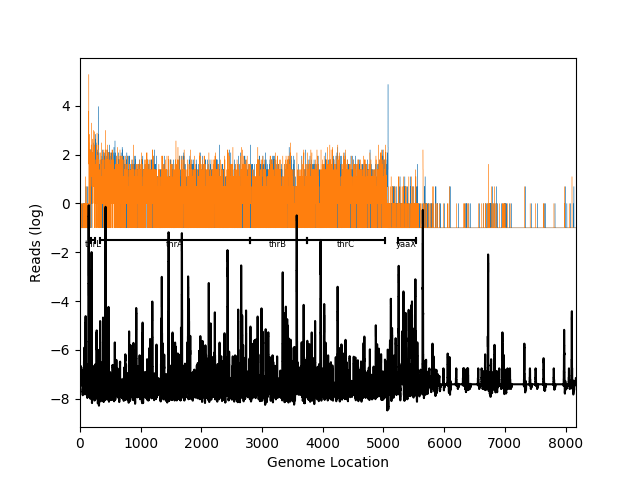
\includegraphics[width=0.4\textwidth]{0_nn_init.png}
    \caption{Example output from supervised learning models for the probability of the initiation class shown in black with read data in blue and orange.  Left: logistic regression. Right: neural network.}
    \label{fig:sup}
\end{figure}

For the neural network implementation, the same parameters were varied as for logistic regression in addition to the network architecture.  Across the range of parameters, 3 hidden layers with 20, 30 and 20 hidden nodes, respectively, seemed to consistently work the best.  Additionally, a moving average window of 15, a sample window of 5, a pad of 0 and oversampling for double the samples provided the best F\textsubscript{1} score.  For both supervised learning methods, many of the incorrectly identified peaks or falsely identified peaks were visually similar.  Most of the poor performance might come from locations that are on the border between classes and could be annotated differently.  Potentially incorporating additional biologic information in labeling initiations and terminations could improve performance and the hand annotation might not be as consistent as it needs to be. 

\begin{table}[H]
  \caption{Recall and precision results from validation and test sets for selected hyperparameters}
  \label{results}
  \centering
  \begin{tabular}{lcccc}
    \toprule
    & \multicolumn{2}{c}{Validation Data} & \multicolumn{2}{c}{Test Data} \\
    \cmidrule(r){2-3} \cmidrule(r){4-5}
    Method & Recall (\%) & Precision (\%) & Recall (\%) & Precision (\%) \\
    \midrule
    DBSCAN & 33.1 & 35.0 & 14.3 & 70.0 \\
    Hidden Markov Model & 23.4 & 70.7 & 12.2 & 42.9 \\
    Logistic Regression & 87.5 & 85.4 & 47.4 & 94.7 \\
    Neural Network & 90.0 & 81.8 & 55.3 & 80.8 \\
    \bottomrule
  \end{tabular}
\end{table}

The results in Table \ref{results} show that the models have been overfit to the training set.  The sensitivity for all methods is lower in the test set compared to the validation showing that none of these methods generalize well to more samples.  The training and validation sets were small so it is not surprising to see performance drop in this case.  Adding more training data would likely reduce the bias and help the methods extend to the entire genome.

\section{Future Work}
Although the results on the test data did not meet expectations, there is some promise in the performance of supervised methods.  One way to improve performance would likely be adding additional training data.  On top of this, additional feature engineering to better encode positional information and the knowledge that locations in the genome will likely be in the same TU as neighboring location could further improve performance.  The class imbalance might also need to be addressed and with additional training data, the majority class could be undersampled while still having enough training examples to train all of the parameters in the model.  Finally, a few other methods could be explored.  A convolutional neural network might improve performance and be able to detect spikes as edges in 1D much like CNNs can do with images in 2D.  Recurrent neural networks also typically offer good performance for sequence data and could be a way to encode the positional information and relation between different locations.

\newpage
\section*{Source Code}
\large{\faGithub} \normalsize \hspace{4pt} All code and data is available on github: \url{www.github.com/tahorst/cs229\_project}

\section*{References}
\small
\begin{enumerate}
\item\label{itm:ecocyc}
"Escherichia coli K-12 substr. MG1655 Transcription-Units" \textit{EcoCyc}. 12 Dec. 2018. https://biocyc.org/ECOLI/class-subs-instances?object=Transcription-Units.

\item\label{itm:lalanne}
Lalanne JB, \textit{et al.} (2018). Evolutionary Convergence of Pathway-Specific Enzyme Expression Stoichiometry. \textit{Cell} 173(3) 749-761.

\item\label{itm:karr}
Karr JR, \textit{et al.} (2012). A whole-cell computational model predicts phenotype from genotype. \textit{Cell} 150(2) 389-401.

\item\label{itm:smote}
Chawla NV, \textit{et al.} (2002). SMOTE: Synthetic Minority Over-sampling Technique. \textit{JAIR} 16
321-357.

\item\label{itm:imblearn}
Lema{{\^i}}tre G, \textit{et al.} (2017). Imbalanced-learn: A Python Toolbox to Tackle the Curse of Imbalanced Datasets in Machine Learning. \textit{Journal of Machine Learning Research} 18 1-5.

\item\label{itm:sklearn}
Pedregosa F, \textit{et al.}. (2011). Scikit-learn: Machine Learning in Python. \textit{Journal of Machine Learning Research} 12 2825-2830.

\item\label{itm:hmmlearn}
(2014). hmmlearn. https://github.com/hmmlearn/hmmlearn.

\item\label{itm:keras}
Chollet F, \textit{et al.} (2015). Keras. https://keras.io.

\item\label{itm:tf}
Abadi M, \textit{et al.} (2015). TensorFlow: Large-Scale Machine Learning on Heterogeneous Systems. https://www.tensorflow.org/.

\end{enumerate}

\end{document}
